\usetikzlibrary{arrows,shapes}
\definecolor{yellow}{rgb}{1.0, 1.0, 0.45} % 255/255/115
\definecolor{dkyellow}{rgb}{0.9, 0.9, 0.0} % % 230/230/0

\definecolor{ltorange}{rgb}{1.0, 0.74, 0.41} % 255/188/105
\definecolor{orange}{rgb}{0.96, 0.50, 0.0} % 246/127/0

\definecolor{ltred}{rgb}{1.0, 0.25, 0.25} % 255/64/64
\definecolor{red}{rgb}{0.79, 0.00, 0.01} % 201/0/3

\definecolor{ltpurple}{rgb}{0.81, 0.57, 1.00} % 206/145/255
\definecolor{purple}{rgb}{0.38, 0.00, 0.68} % 97/1/175

\definecolor{ltblue}{rgb}{0.2, 0.73, 1.0} % 51/187/255
\definecolor{blue}{rgb}{0.12, 0.43, 0.59} % 30/110/150

\definecolor{ltltgreen}{rgb}{0.7, 1.00, 0.7} % 96/204/14
\definecolor{ltgreen}{rgb}{0.37, 0.80, 0.05} % 96/204/14
\definecolor{green}{rgb}{0.23, 0.49, 0.03} % 59/125/8
  
\definecolor{dkslate}{rgb}{0.18, 0.21, 0.28} % 47/53/72
\definecolor{mdslate}{rgb}{0.45, 0.50, 0.68} % 114/127/173
\definecolor{ltslate}{rgb}{0.85, 0.88, 0.95} % 216/225/229

\tikzstyle{level0} = [rectangle, 
                      minimum width=5em, 
                      text centered,
                      rounded corners=0.75em,
                      minimum height=2em,
                      very thick,
                      draw=blue!80!black,
                      top color=ltblue!50!white,
                      bottom color=blue]
\tikzstyle{level1} = [rectangle, 
                      minimum width=5em, 
                      text centered,
                      rounded corners=0.75em,
                      minimum height=2em,
                      very thick,
                      draw=green!80!black,
                      top color=ltgreen!50!white,
                      bottom color=green]
\tikzstyle{level2} = [rectangle, 
                      minimum width=5em, 
                      text centered,
                      rounded corners=0.75em,
                      minimum height=2em,
                      very thick,
                      draw=orange!80!black,
                      top color=ltorange!50!white,
                      bottom color=orange]
\tikzstyle{level3} = [rectangle, 
                      minimum width=5em, 
                      text centered,
                      rounded corners=0.75em,
                      minimum height=2em,
                      very thick,
                      draw=red!80!black,
                      top color=ltred!50!white,
                      bottom color=red]
\begin{center}
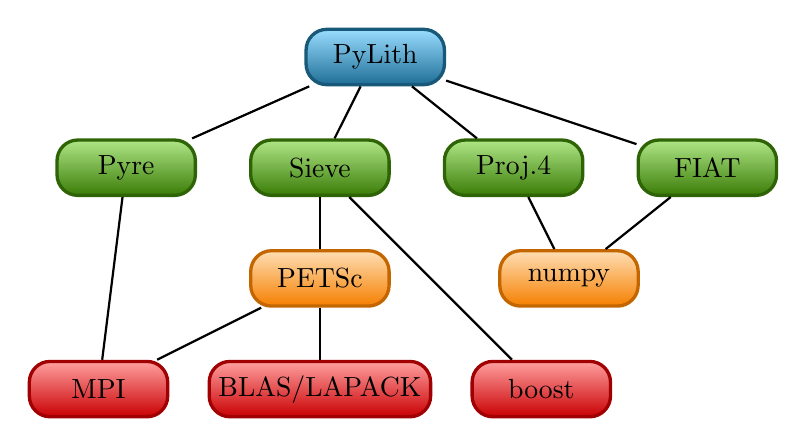
\begin{tikzpicture}[node distance=7.0em,
                    arrowto/.style={-, thick}]
  % Level 0
  \node (pylith) [level0] {PyLith};

  % Level 1
  \node (sieve) [level1, below of=pylith, xshift=-2em, yshift=+3em] {Sieve};
  \node (pyre) [level1, left of=sieve] {Pyre};
  \node (proj4) [level1, right of=sieve] {Proj.4};
  \node (fiat) [level1, right of=proj4] {FIAT};

  \path (pylith) edge[arrowto] (pyre);
  \path (pylith) edge[arrowto] (sieve);
  \path (pylith) edge[arrowto] (proj4);
  \path (pylith) edge[arrowto] (fiat);

  % Level 2
  \node (petsc) [level2, below of=sieve, yshift=+3em] {PETSc};
  \node (numpy) [level2, right of=petsc, xshift=2em] {numpy};

  \path (sieve) edge[arrowto] (petsc);
  \path (fiat) edge[arrowto] (numpy);
  \path (proj4) edge[arrowto] (numpy);

  % Level 3
  \node (blas) [level3, below of=petsc, yshift=+3em] {BLAS/LAPACK};
  \node (mpi) [level3, left of=blas, xshift=-1em] {MPI};
  \node (boost) [level3, right of=blas, xshift=1em] {boost};

  \path (pyre) edge[arrowto] (mpi);
  \path (petsc) edge[arrowto] (mpi);
  \path (petsc) edge[arrowto] (blas);
  \path (sieve) edge[arrowto] (boost);


\end{tikzpicture}
\end{center}
\vfill
